\chapter{Evaluation}
\section{Correctness of algorithms}
The correctness of the parsing, matching, and verification algorithms are verified using unit tests. Some test cases are based on subsets of the pre-defined proof systems---natural deduction, Curry type assignment for the lambda calculus, and the sequent calculus system LK---while other test cases are based on variously modified rules from these systems and designed to catch edge cases. Some test cases based on the lambda calculus are taken from the course notes for the Type Systems module at Imperial \cite{van-bakel:2022}. Some test cases based on the system LK are taken from a set of online logic notes \cite{sequent}.

There is a high degree of confidence in the matching and verification algorithms, since they are based on custom data structures independent of the user input. To identify further edge cases in the parsing algorithm and determine how well the parsing algorithm adapts to a wide range of user inputs, the parsing algorithm is tested against extensions of the pre-defined systems and brand new proof systems.

\subsection{Lambda calculus with pairs}
The syntaxes of $\lambda$-terms and Curry types are extended with the following constructors \cite{van-bakel:2022}:
\begin{align*}
    M, N &\Coloneqq \ldots \alt \langle M, N \rangle \alt \textsf{left}(M) \alt \textsf{right}(M) \\
    A, B &\Coloneqq \ldots \alt (A \times B)
\end{align*}
The three new constructors for $\lambda$-terms are accompanied with the following extensions to the type assignment rules:
\[
    (\textit{Pair}): \frac{\Gamma \vdash M: A \quad \Gamma \vdash N: B}{\Gamma \vdash \langle M, N \rangle: (A \times B)} \quad (\textsf{left}): \frac{\Gamma \vdash M: (A \times B)}{\Gamma \vdash \textsf{left}(M): A} \quad (\textsf{right}): \frac{\Gamma \vdash M: (A \times B)}{\Gamma \vdash \textsf{right}(M): B} 
\]
Although the user can type ``left'' and ``right'' for the two constructors, they will be rendered in math mode in \LaTeX{} as $left$ and $right$, which do not look the nicest. Prior to testing with the lambda calculus with pairs, the parsing algorithm can only handle \LaTeX{} commands that do not take any arguments, such as ``\textbackslash Gamma'' for $\Gamma$ and ``\textbackslash varphi'' for $\varphi$. The lambda calculus with pairs motivates extending the parsing algorithm to parse \LaTeX{} commands as literal strings. In this case, ``\textbackslash textsf{left}(M)'' should be rendered as $\textsf{left}(M)$ and parsed into \lstinline{Token}s as
\begin{center}
    \lstinline|[Terminal("\textsf{left}"), Terminal("("), NonTerminal(...), Terminal(")")]|
\end{center}
A correct derivation using all three newly added constructors and type assignment rules is shown in \Cref{evaluation:lambda-with-pairs}.
\begin{figure}[!htbp]
    \centering
    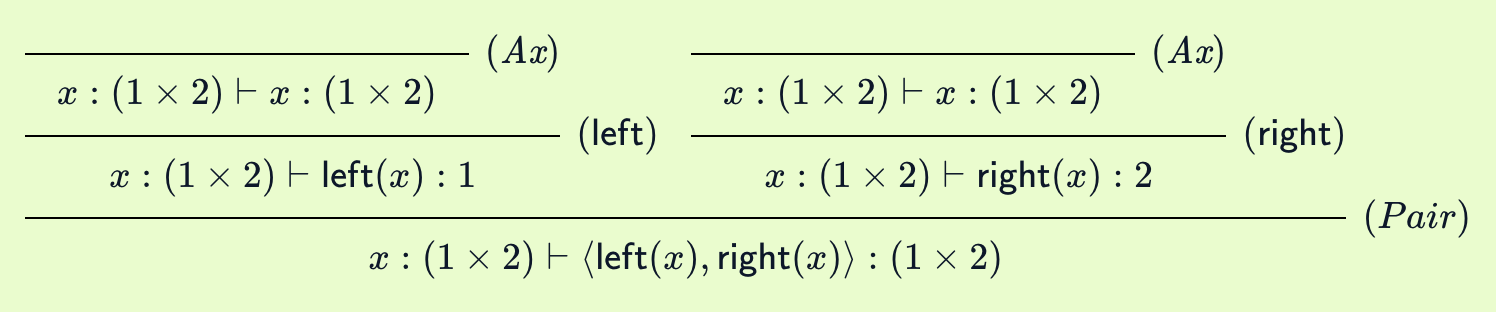
\includegraphics[width=0.7\textwidth]{evaluation/lambda-with-pairs.png}
    \caption{A correct derivation }
    \label{evaluation:lambda-with-pairs}
\end{figure}

\subsection{\lbm{}}
The calculus \lbm{} as presented by Curien and Herbelin \cite{curien-herbelin:2000} defines three types of terms \cite{van-bakel:2024}:
\begin{align*}
    c &\Coloneqq \langle t | e \rangle &(\textit{commands}) \\
    t &\Coloneqq x \alt (\lambda x. t) \alt (\mu \beta. c) &(\textit{terms}) \\
    e &\Coloneqq \alpha \alt (t \cdot e) \alt (\tilde{\mu}x. c) &(\textit{environments})
\end{align*}
where $x$ can be any symbol from an infinite list of term variables $a, b, c, \ldots, x, y, z \ldots$. \todo{What are $\alpha$ and $\beta$?} \lbm{} defines three kinds of statements, each typing a different syntactic category:
\begin{align*}
    \text{Statement} \Coloneqq{} &c: \Gamma \vdash \Delta &(\textit{commands}) \\
    |\  &\Gamma \vdash t: A \alt \Delta &(\textit{terms}) \\
    |\  &\Gamma \alt e: A \vdash \Delta &(\textit{environments})
\end{align*}
where $A$ represents a Curry type, while $\Gamma$ and $\Delta$ represent a set of variable type assignments. The type assignment rules are defined as follows:
\[
    (\textit{cut}): \frac{\Gamma \vdash t: A \alt \Delta \quad \Gamma \alt e: A \vdash \Delta}{\langle t|e \rangle: \Gamma \vdash \Delta}
\]

\begin{center}
    \begin{minipage}{.4\textwidth}
        \begingroup
        \addtolength{\jot}{1em}
        \begin{align*}
            (Ax_R)&: \frac{}{\Gamma, x: A \vdash x: A \alt \Delta} \\
            (\to R)&: \frac{\Gamma, x: A \vdash t: B \alt \Delta}{\Gamma \vdash (\lambda x. t): (A \to B) \alt \Delta} \\
            (\mu)&: \frac{c: \Gamma \vdash \alpha: A, \Delta}{\Gamma \vdash (\mu \alpha. c): A \alt \Delta}
        \end{align*}
        \endgroup
    \end{minipage}%
    \begin{minipage}{.4\textwidth}
        \begingroup
        \addtolength{\jot}{1em}
        \begin{align*}
            (Ax_L)&: \frac{}{\Gamma \alt \alpha: A \vdash \alpha: A, \Delta} \\
            (\to L)&: \frac{\Gamma \vdash t: A \alt \Delta \quad \Gamma \alt e: B \vdash \Delta}{\Gamma \alt (t \cdot e): (A \to B) \vdash \Delta} \\
            (\tilde{\mu})&: \frac{c: \Gamma, x: A \vdash \Delta}{\Gamma \alt (\tilde{\mu}x. c): A \vdash \Delta}
        \end{align*}
        \endgroup
    \end{minipage}
\end{center}